%%%%%%%%%%%%%%%%%%%%%%%%%%%%%%%%%%%%%%%%%
% fphw Assignment
% LaTeX Template
% Version 1.0 (27/04/2019)
%
% This template originates from:
% https://www.LaTeXTemplates.com
%
% Authors:
% Class by Felipe Portales-Oliva (f.portales.oliva@gmail.com) with template 
% content and modifications by Vel (vel@LaTeXTemplates.com)
%
% Template (this file) License:
% CC BY-NC-SA 3.0 (http://creativecommons.org/licenses/by-nc-sa/3.0/)
%
%%%%%%%%%%%%%%%%%%%%%%%%%%%%%%%%%%%%%%%%%

%----------------------------------------------------------------------------------------
%	PACKAGES AND OTHER DOCUMENT CONFIGURATIONS
%----------------------------------------------------------------------------------------

\documentclass[
  12pt,
  %fleqn, % Default font size, values between 10pt-12pt are allowed
  %letterpaper, % Uncomment for US letter paper size
  %spanish, % Uncomment for Spanish
]{fphw}

% Template-specific packages
\usepackage[utf8]{inputenc} % Required for inputting international characters
\usepackage[T1]{fontenc} % Output font encoding for international characters
\usepackage{mathpazo} % Use the Palatino font

\usepackage{graphicx} % Required for including images

\usepackage{booktabs} % Required for better horizontal rules in tables
\usepackage{listings} % Required for insertion of code
\usepackage{enumerate} % To modify the enumerate environment
\usepackage{enumitem}
\usepackage{amsmath}
\usepackage{mathtools,amsthm}
\usepackage{float}
\usepackage{listings}
\usepackage{pdfpages}
\usepackage{hyperref}
\usepackage{amssymb}
\usepackage{mathtools}

\lstdefinelanguage{R}{
  keywords={if, else, repeat, while, function, for, in, next, break},
  otherkeywords={TRUE, FALSE, NULL, NA, Inf, NaN},
  sensitive=true,
  morecomment=[l]\#,
  morestring=[b]",
}

\newcommand{\E}{\mathbb{E}}
\newcommand{\Var}{\operatorname{Var}}
\newcommand{\R}{\mathbb{R}}
\newcommand{\norm}[1]{\left\lVert #1 \right\rVert}


%----------------------------------------------------------------------------------------
%	ASSIGNMENT INFORMATION
%----------------------------------------------------------------------------------------

\title{Homework \#8} % Assignment title

\author{Shizhe Zhang} % Student name

\date{\today} % Due date

\institute{University of California, Berkeley \\ Department of Statistics} % Institute or school name

\class{EECS 227AT} % Course or class name

\professor{Gireeja Ranade} % Professor or teacher in charge of the assignment

%----------------------------------------------------------------------------------------

\begin{document}

\maketitle % Output the assignment title, created automatically using the information in the custom commands above

%----------------------------------------------------------------------------------------
%	ASSIGNMENT CONTENT
%----------------------------------------------------------------------------------------

\section*{Problem 1. Convergence of Gradient Descent for Ridge Regression}

Let $A \in \mathbb{R}^{m \times n}$, $\vec{y} \in \mathbb{R}^{m}$, and $\lambda > 0$. Consider a slight variation of the ridge regression problem where the least squares loss is normalized by the number of data points:

\[
\min_{\vec{x}\in\mathbb{R}^{n}} f_\lambda(\vec{x})
\]

where

\[
f_\lambda(\vec{x}) \triangleq \frac12 \left\{ \frac1m \|A\vec{x}-\vec{y}\|_2^2 + \lambda \|\vec{x}\|_2^2
\right\}.
\tag{1}
\]

In this problem, we will examine the behavior of gradient descent (GD) on this problem, and in particular the interplay between the learning rate $\eta > 0$ and regularization parameter $\lambda > 0$ in determining convergence.


\textbf{(a)}
Show that the unique solution to the problem in Equation (1) is

\[
\vec{x}_\lambda^\star = (A^\top A + \lambda m I)^{-1} A^\top \vec{y}.
\tag{2}
\]

\textbf{(b)}
Show that the GD update

\[
\vec{x}_{t+1} = \vec{x}_t - \eta \left( \frac1m A^\top(A\vec{x}_t - \vec{y}) + \lambda \vec{x}_t
\right)
\tag{3}
\]

can be rearranged into the form

\[
\vec{x}_{t+1}-\vec{x}_\lambda^\star = \left( I - \eta \left( \frac{A^\top A}{m} + \lambda I \right) \right) (\vec{x}_t-\vec{x}_\lambda^\star).
\tag{4}
\]

Use this to show that

\[
\vec{x}_t-\vec{x}_\lambda^\star = \left( I - \eta \left( \frac{A^\top A}{m} + \lambda I \right) \right)^t (\vec{x}_0-\vec{x}_\lambda^\star)
\tag{5}
\]

for every positive integer $t$.

\textbf{(c)}
We now discuss the insight that the SVD can give us regarding the convergence of GD. Let

\[
A = U\Sigma V^\top
\]

be a full SVD of $A$. Let

\[
\vec{z}_t = V^\top \vec{x}_t
\]

and

\[
\vec{z}_\lambda^\star = V^\top \vec{x}_\lambda^\star.
\]

Show that

\[
\vec{z}_t - \vec{z}_\lambda^\star
=
\left(
I - \eta \left( \frac{\Sigma^\top\Sigma}{m} + \lambda I \right) \right)^t (\vec{z}_0-\vec{z}_\lambda^\star).  \tag{6}
\]

Moreover, show that for each $i \in \{1,\dots,n\}$,

\[
(z_t)_i - (z_\lambda^\star)_i = \left( 1-\eta\left(\frac{\sigma_i\{A\}^2}{m}+\lambda\right) \right)^t
\left((z_0)_i-(z_\lambda^\star)_i\right) \tag{7}
\]

where $\sigma_i\{A\}$ is the $i$th largest singular value of $A$.

This shows that the rate of convergence of $\vec{z}_t$ to $\vec{z}_\lambda^\star$ along the $i$th component is influenced by the interaction between $\sigma_i\{A\}$, $\lambda$, and $\eta$, but critically no other singular values. Thus, one considers the $V$ basis to be the “natural” basis for thinking about GD for ridge regression.

\textbf{(d)}
Show that

\[
\lim_{t\to\infty} \vec{z}_t = \vec{z}_\lambda^\star
\]

for all initializations $\vec{x}_0 = V\vec{z}_0$ if and only if

\[
\max_{i\in\{1,\dots,n\}}
\left|
1-\eta\left(\frac{\sigma_i\{A\}^2}{m}+\lambda\right)
\right| < 1.
\tag{8}
\]

Use this to show that GD converges for all initializations $\vec{x}_0$ if and only if

\[
\eta
\in
\left(
0,
\frac{2m}{\sigma_{\max}\{A\}^2+\lambda m}
\right)
\tag{9}
\]

where $\sigma_{\max}\{A\}=\sigma_1\{A\}$ is the largest singular value of $A$.

\textbf{(e) (OPTIONAL)}
One way we can derive an “optimal” learning rate $\eta^\star$ is to minimize the largest rate of convergence:

\[
\eta^\star \in \arg\min_{\eta\in\mathbb{R}} \max_{i\in\{1,\dots,n\}} \left| 1-\eta \left( \frac{\sigma_i\{A\}^2}{m}+\lambda \right) \right|.  \tag{10}
\]

One important property of $\eta^\star$ is that it makes the rates of convergence

\[ \left| 1-\eta \left( \frac{\sigma_i\{A\}^2}{m}+\lambda \right) \right| \]

associated with the largest and smallest singular values of $A$ equal.

Use this property to show that

\[
\eta^\star
=
\frac{2m}
{\sigma_{\max}\{A\}^2
+
\sigma_{\min}\{A\}^2
+
2\lambda m}.
\tag{11}
\]

NOTE: There are several useful notions of optimal learning rate; this is just one of them.

\textbf{(f)}
The attached notebook, \texttt{gd\_convergence.ipynb}, will examine the computational aspects of GD on ridge regression. Implement the GD and stochastic gradient descent (SGD) functions at the top of the notebook, which are marked with TODOs.

\textbf{(g)}
Click through the notebook and run the sections $n=1$, $n=2$, and $n\gg2$. Change the values of $\lambda$ and $\eta$ and re-run the cells a few times. Write down your observations about how the convergence of GD works under different values of $\lambda$ and $\eta$.

\textbf{(h)}
In the sections $n=1$, $n=2$, and $n\gg2$, change the calls to GD to instead call SGD. Write down your observations about how the convergence of SGD works under different values of $\lambda$ and $\eta$. Compare the behavior of GD and SGD.

\textbf{(i)}
You might have noticed that if we think of convergence in the “last iterate” sense, i.e.,
\[
\lim_{T\to\infty} \vec{x}_T = \vec{x}_\lambda^\star,
\]
then SGD rarely converges.

This is because even if we reach the global optimum, the gradient estimate used by SGD is in general nonzero, and so the iterates end up bouncing around near the optimum.

Another different, weaker notion of convergence under which one might show that SGD actually does converge is convergence “in time average”, i.e.,
$
\lim_{T\to\infty} \bar{x}_T = \vec{x}_\lambda^\star
$
where
$ \bar{x}_T \triangleq \frac1T \sum_{t=1}^T x_t. $

Visualize this by adding the argument \texttt{time\_avg=True} to each plotting function; the plot will now visualize the sequence of $\bar{x}_t$. Re-run the notebook. Write down your observations, especially regarding the stability of SGD and convergence in the last-iterate sense versus the time-average sense.

\subsection*{Answer}

\textbf{(a)}

We consider

\[
f_\lambda(\vec{x})= \frac12 \left( \frac1m\|A\vec{x}-\vec{y}\|_2^2 + \lambda\|\vec{x}\|_2^2 \right).
\]

First compute the gradient.

\[
\nabla_x \|A\vec{x}-\vec{y}\|_2^2 = 2A^\top(A\vec{x}-\vec{y})
\]

Thus

\[
\nabla f_\lambda(\vec{x}) = \frac{1}{m}A^\top(A\vec{x}-\vec{y})+\lambda \vec{x}.
\]

Setting the gradient to zero,

\[
\frac1mA^\top(A\vec{x}-\vec{y})+\lambda\vec{x}=0.
\]

Multiplying both sides by \(m\),

\[
A^\top A\vec{x}-A^\top\vec{y}+\lambda m\vec{x}=0.
\]

Rearranging,

\[
(A^\top A+\lambda mI)\vec{x}=A^\top\vec{y}.
\]

Since \(A^\top A+\lambda mI\) is positive definite for \(\lambda>0\), it is invertible, giving

\[
\vec{x}_\lambda^\star
=
(A^\top A+\lambda mI)^{-1}A^\top\vec{y}.
\]

\textbf{(b)}

The GD update is

\[
\vec{x}_{t+1}
=
\vec{x}_t
-
\eta
\left(
\frac1mA^\top(A\vec{x}_t-\vec{y})
+
\lambda\vec{x}_t
\right).
\]

Rewrite the update:

\[
\vec{x}_{t+1}
=
\vec{x}_t
-
\eta
\left(
\frac{A^\top A}{m}\vec{x}_t
-
\frac{A^\top \vec{y}}{m}
+
\lambda \vec{x}_t
\right).
\]

Using the optimality condition

\[
(A^\top A+\lambda mI)\vec{x}_\lambda^\star
=
A^\top\vec{y},
\]

we obtain

\[
\frac{A^\top\vec{y}}{m}
=
\left(\frac{A^\top A}{m}+\lambda I\right)\vec{x}_\lambda^\star.
\]

Substituting,

\[
\vec{x}_{t+1}
=
\vec{x}_t
-
\eta
\left(\frac{A^\top A}{m}+\lambda I\right)
(\vec{x}_t-\vec{x}_\lambda^\star).
\]

Thus

\[
\vec{x}_{t+1}-\vec{x}_\lambda^\star
=
\left(I-\eta\left(\frac{A^\top A}{m}+\lambda I\right)\right)
(\vec{x}_t-\vec{x}_\lambda^\star).
\]

Applying the recursion repeatedly gives

\[
\vec{x}_t-\vec{x}_\lambda^\star
=
\left(I-\eta\left(\frac{A^\top A}{m}+\lambda I\right)\right)^t
(\vec{x}_0-\vec{x}_\lambda^\star).
\]

\textbf{(c)}

Then

\[
A^\top A = V\Sigma^\top\Sigma V^\top.
\]

Define

\[
\vec{z}_t=V^\top\vec{x}_t, \qquad
\vec{z}_\lambda^\star=V^\top\vec{x}_\lambda^\star.
\]

Multiplying equation (5) by \(V^\top\),

\[
\vec{z}_t-\vec{z}_\lambda^\star
=
V^\top
\left(I-\eta\left(\frac{A^\top A}{m}+\lambda I\right)\right)^t
V
(\vec{z}_0-\vec{z}_\lambda^\star).
\]

Since

\[
V^\top A^\top A V=\Sigma^\top\Sigma,
\]

we obtain

\[
\vec{z}_t-\vec{z}_\lambda^\star
=
\left(I-\eta\left(\frac{\Sigma^\top\Sigma}{m}+\lambda I\right)\right)^t
(\vec{z}_0-\vec{z}_\lambda^\star).
\]

Because \(\Sigma^\top\Sigma\) is diagonal with entries \(\sigma_i(A)^2\),

\[
(z_t)_i-(z_\lambda^\star)_i
=
\left(
1-\eta\left(\frac{\sigma_i(A)^2}{m}+\lambda\right)
\right)^t
((z_0)_i-(z_\lambda^\star)_i).
\]

Thus each coordinate converges independently.

\textbf{(d)}

From part (c),

\[
(z_t)_i-(z_\lambda^\star)_i
=
\left(
1-\eta\left(\frac{\sigma_i(A)^2}{m}+\lambda\right)
\right)^t
((z_0)_i-(z_\lambda^\star)_i).
\]

For convergence as \(t\to\infty\), we require

\[
\left|
1-\eta\left(\frac{\sigma_i(A)^2}{m}+\lambda\right)
\right|<1
\]

for all \(i\).

This gives

\[
-1
<
1-\eta\left(\frac{\sigma_i(A)^2}{m}+\lambda\right)
<
1.
\]

The right inequality gives

\[
\eta>0.
\]

The left inequality gives

\[
\eta
<
\frac{2}{\frac{\sigma_i(A)^2}{m}+\lambda}.
\]

For all \(i\), the most restrictive condition occurs at
\(\sigma_{\max}(A)\). Thus

\[
\eta
<
\frac{2}{\frac{\sigma_{\max}(A)^2}{m}+\lambda}.
\]

Therefore GD converges for all initializations if

\[
\eta\in
\left(
0,
\frac{2m}{\sigma_{\max}(A)^2+\lambda m}
\right).
\]


\textbf{(e)}

The optimal learning rate equalizes the largest and smallest convergence factors:

\[
\left|
1-\eta\left(\frac{\sigma_{\max}(A)^2}{m}+\lambda\right)
\right|
=
\left|
1-\eta\left(\frac{\sigma_{\min}(A)^2}{m}+\lambda\right)
\right|.
\]

This yields

\[
1-\eta\left(\frac{\sigma_{\max}^2}{m}+\lambda\right)
=
-
\left(
1-\eta\left(\frac{\sigma_{\min}^2}{m}+\lambda\right)
\right).
\]

Simplifying,

\[
2
=
\eta
\left(
\frac{\sigma_{\max}^2+\sigma_{\min}^2}{m}+2\lambda
\right).
\]

Thus

\[
\eta^\star
=
\frac{2}
{\frac{\sigma_{\max}^2+\sigma_{\min}^2}{m}+2\lambda}
=
\frac{2m}{\sigma_{\max}^2+\sigma_{\min}^2+2\lambda m}.
\]

\textbf{(g)}

I re-ran the notebook for $n=1,2,10$ while varying both $\lambda$ and $\eta$.
The empirical behavior matches the theory from part (d):

\begin{itemize}
  \item For GD, increasing $\eta$ generally speeds up convergence until a stability boundary is crossed.
  \item For moderate dimensions ($n=1,2$), GD converged reliably for a wide range of step sizes around $\eta^\star$.
  \item For higher dimension ($n=10$), the instability is more visible: with small regularization ($\lambda=0.01$), using a large step (e.g., $\eta\approx 1.5\eta^\star$) caused divergence (overflow/inf in the iterate error).
  \item Increasing $\lambda$ improves conditioning and makes GD behavior more stable across step sizes.
\end{itemize}

In the convergence plots, GD trajectories are smooth and nearly geometric on a log scale, especially in the $V$ basis, consistent with coordinate-wise contraction factors.

\textbf{(h)}

After replacing GD calls with SGD and sweeping $\lambda,\eta$ again, the behavior changes qualitatively:

\begin{itemize}
  \item SGD last iterates are noisy and oscillatory; they do not settle to a single point even when objective values are small.
  \item Larger $\eta$ increases variance of the iterates and can lead to severe instability/divergence in high dimension (for $n=10$ and small $\lambda$, large-step runs produced NaNs).
  \item Compared with GD, SGD is less stable at the same nominal scale of $\eta$, and convergence diagnostics based on $\|x_t-x_\lambda^\star\|$ are much worse for last iterates.
  \item Stronger regularization ($\lambda$ larger) damps noise somewhat, but does not remove last-iterate oscillation.
\end{itemize}

So GD gives fast and clean deterministic convergence, while SGD trades that for noisy but inexpensive updates.

\textbf{(i)}

Using the plotting functions with \texttt{time\_avg=True} confirms the expected phenomenon:

\begin{itemize}
  \item Last-iterate SGD remains jittery around the optimum in both standard and $V$ bases.
  \item Time-averaged SGD, $\bar{x}_t$, is much more stable and trends downward in error/objective gap, often by one or more orders of magnitude relative to last-iterate error.
  \item This effect is strongest in noisy/high-dimensional settings ($n=10$), where averaging converts highly variable trajectories into steadily improving ones.
\end{itemize}

Therefore, for SGD in this problem, ``convergence in last iterate'' is typically poor, while ``convergence in time average'' is the practically meaningful notion.
%%%%%%%%%%%%%%%%%%%%%%%%%%%%%%%%%%%%%%%%%%%%%%%%%%%%%%%%%%%%
\newpage
\section*{2. Convexity of Rank 1 Matrices}

First, consider the set of all $2\times2$ matrices with diagonal elements $(1,2)$:

\[
S = \left\{ \begin{bmatrix} 1 & x\\ y & 2 \end{bmatrix} \mid x,y\in\mathbb{R} \right\}.  \tag{12}
\]

\textbf{(a)} Is set $S$ convex? If so, provide a proof, and if not, provide a counterexample.

\textbf{(b)} Suppose we now wish to define $S_1\subset S$, the set of all rank-1 matrices in $S$. Write out conditions on $x$ and $y$ to define $S_1$ explicitly.

\textbf{(c)} Is set $S_1$ convex? If so, provide a proof, and if not, provide a counterexample.

\textbf{(d)} Consider the optimization problem

\[
\min_{A\in S_1} \|A\|_F^2 \tag{13}
\]

which is equivalent to

\[
\min_{A\in S} \|A\|_F^2 \tag{14}
\]

subject to

\[
\text{rank}(A)=1.  \tag{15}
\]

Is this optimization problem convex?

\subsection*{Answer}

First consider the set

\[
S =
\left\{
\begin{bmatrix}
1 & x \\
y & 2
\end{bmatrix}
\;\middle|\;
x,y \in \mathbb{R}
\right\}.
\]

\textbf{(a)}

Yes, $S$ is convex.

Let

\[
A =
\begin{bmatrix}
1 & x_1 \\
y_1 & 2
\end{bmatrix},
\quad
B =
\begin{bmatrix}
1 & x_2 \\
y_2 & 2
\end{bmatrix}
\]

be two matrices in $S$. Let $\theta \in [0,1]$.

Consider the convex combination

\[
\theta A + (1-\theta)B.
\]

We compute

\[
\theta A + (1-\theta)B
=
\begin{bmatrix}
\theta + (1-\theta) & \theta x_1 + (1-\theta)x_2 \\
\theta y_1 + (1-\theta)y_2 & 2\theta + 2(1-\theta)
\end{bmatrix}.
\]

Simplifying,

\[
=
\begin{bmatrix}
1 & \theta x_1 + (1-\theta)x_2 \\
\theta y_1 + (1-\theta)y_2 & 2
\end{bmatrix}.
\]

Since $\theta x_1 + (1-\theta)x_2$ and $\theta y_1 + (1-\theta)y_2$ are real numbers, the resulting matrix is still in $S$. Therefore $S$ is convex.

\textbf{(b)}

Let

\[
A =
\begin{bmatrix}
1 & x \\
y & 2
\end{bmatrix}.
\]

For a $2\times2$ matrix to have rank $1$, its determinant must be zero. Thus

\[
\det(A) = 0.
\]

Compute the determinant:

\[
\det(A) = (1)(2) - xy = 2 - xy.
\]

Setting this equal to zero,

\[
xy = 2.
\]

\[ S_1 = \left\{ \begin{bmatrix} 1 & x \\ y & 2 \end{bmatrix} \;\middle|\; xy = 2 \right\}.  \]


\textbf{(c)}

The set $S_1$ is not convex.

Consider the matrices

\[
A_1 =
\begin{bmatrix}
1 & 1 \\
2 & 2
\end{bmatrix},
\quad
A_2 =
\begin{bmatrix}
1 & 2 \\
1 & 2
\end{bmatrix}.
\]

Both satisfy $xy = 2$, so they belong to $S_1$.

Now consider their average:

\[
A = \frac{1}{2}A_1 + \frac{1}{2}A_2
=
\begin{bmatrix}
1 & 1.5 \\
1.5 & 2
\end{bmatrix}.
\]

For this matrix

\[
xy = (1.5)(1.5) = 2.25 \neq 2.
\]

Thus $A \notin S_1$, meaning the convex combination of two matrices in $S_1$ is not necessarily in $S_1$. Therefore $S_1$ is not convex.

\textbf{(d)}

The optimization problem is

\[
\min_{A \in S_1} \|A\|_F^2.
\]

\[
\|A\|_F^2 = \sum_{i,j} A_{ij}^2,
\]

which is a convex function.

However, the feasible set $S_1$ is not convex (from part (c)) because of the rank constraint.

Thus, this  problem is not convex.

%%%%%%%%%%%%%%%%%%%%%%%%%%%%%%%%%%%%%%%%%%%%%%%%%%%%%%%%%%%%
\newpage
\section*{3. Positive Semi-Definite Cone}

Let $A,B\in\mathbb{R}^{n\times n}$ be symmetric positive semidefinite matrices.

Show that
\[
\langle A,B\rangle \ge 0
\]

where

\[
\langle A,B\rangle = \mathrm{tr}(AB^\top)
\]

is the usual inner product on matrices.

HINT: Try an eigendecomposition of
$
B=\sum_{i=1}^n \lambda_i u_i u_i^\top
$
and use the trace formula of the inner product.

\subsection*{Answer}


Since $B$ is symmetric, we have $B^\top = B$, so

\[
\langle A,B\rangle = \mathrm{tr}(AB).
\]

Because $B$ is positive semidefinite, it admits the eigendecomposition

\[
B = \sum_{i=1}^{n} \lambda_i u_i u_i^\top
\]

where $\lambda_i \ge 0$ are the eigenvalues and $\{u_i\}$ are orthonormal eigenvectors.

Substituting this into the inner product,

\[
\langle A,B\rangle
=
\mathrm{tr}\left(A \sum_{i=1}^{n} \lambda_i u_i u_i^\top\right).
\]

Using linearity of the trace,

\[
=
\sum_{i=1}^{n} \lambda_i \mathrm{tr}(A u_i u_i^\top).
\]

Using the cyclic property of trace,

\[
\mathrm{tr}(A u_i u_i^\top) = \mathrm{tr}(u_i^\top A u_i) = u_i^\top A u_i.
\]

Thus

\[
\langle A,B\rangle
=
\sum_{i=1}^{n} \lambda_i \, u_i^\top A u_i.
\]

Since $A$ is positive semidefinite,

\[
u_i^\top A u_i \ge 0
\]

for all $i$, and since $\lambda_i \ge 0$, every term in the sum is nonnegative. Therefore

\[
\langle A,B\rangle \ge 0.
\]

Hence, the inner product of two symmetric positive semidefinite matrices is always nonnegative.

%%%%%%%%%%%%%%%%%%%%%%%%%%%%%%%%%%%%%%%%%%%%%%%%%%%%%%%%%%%%
\newpage
\section*{4. Visualizing the Dual Problem}

Use the associated \href{https://colab.research.google.com/drive/1UxmJhZRjMUeEN7XkzIh8jdUES8iBQxBP?usp=sharing}{Google Colab notebook}; complete the code where designated and answer the questions given in the space provided.

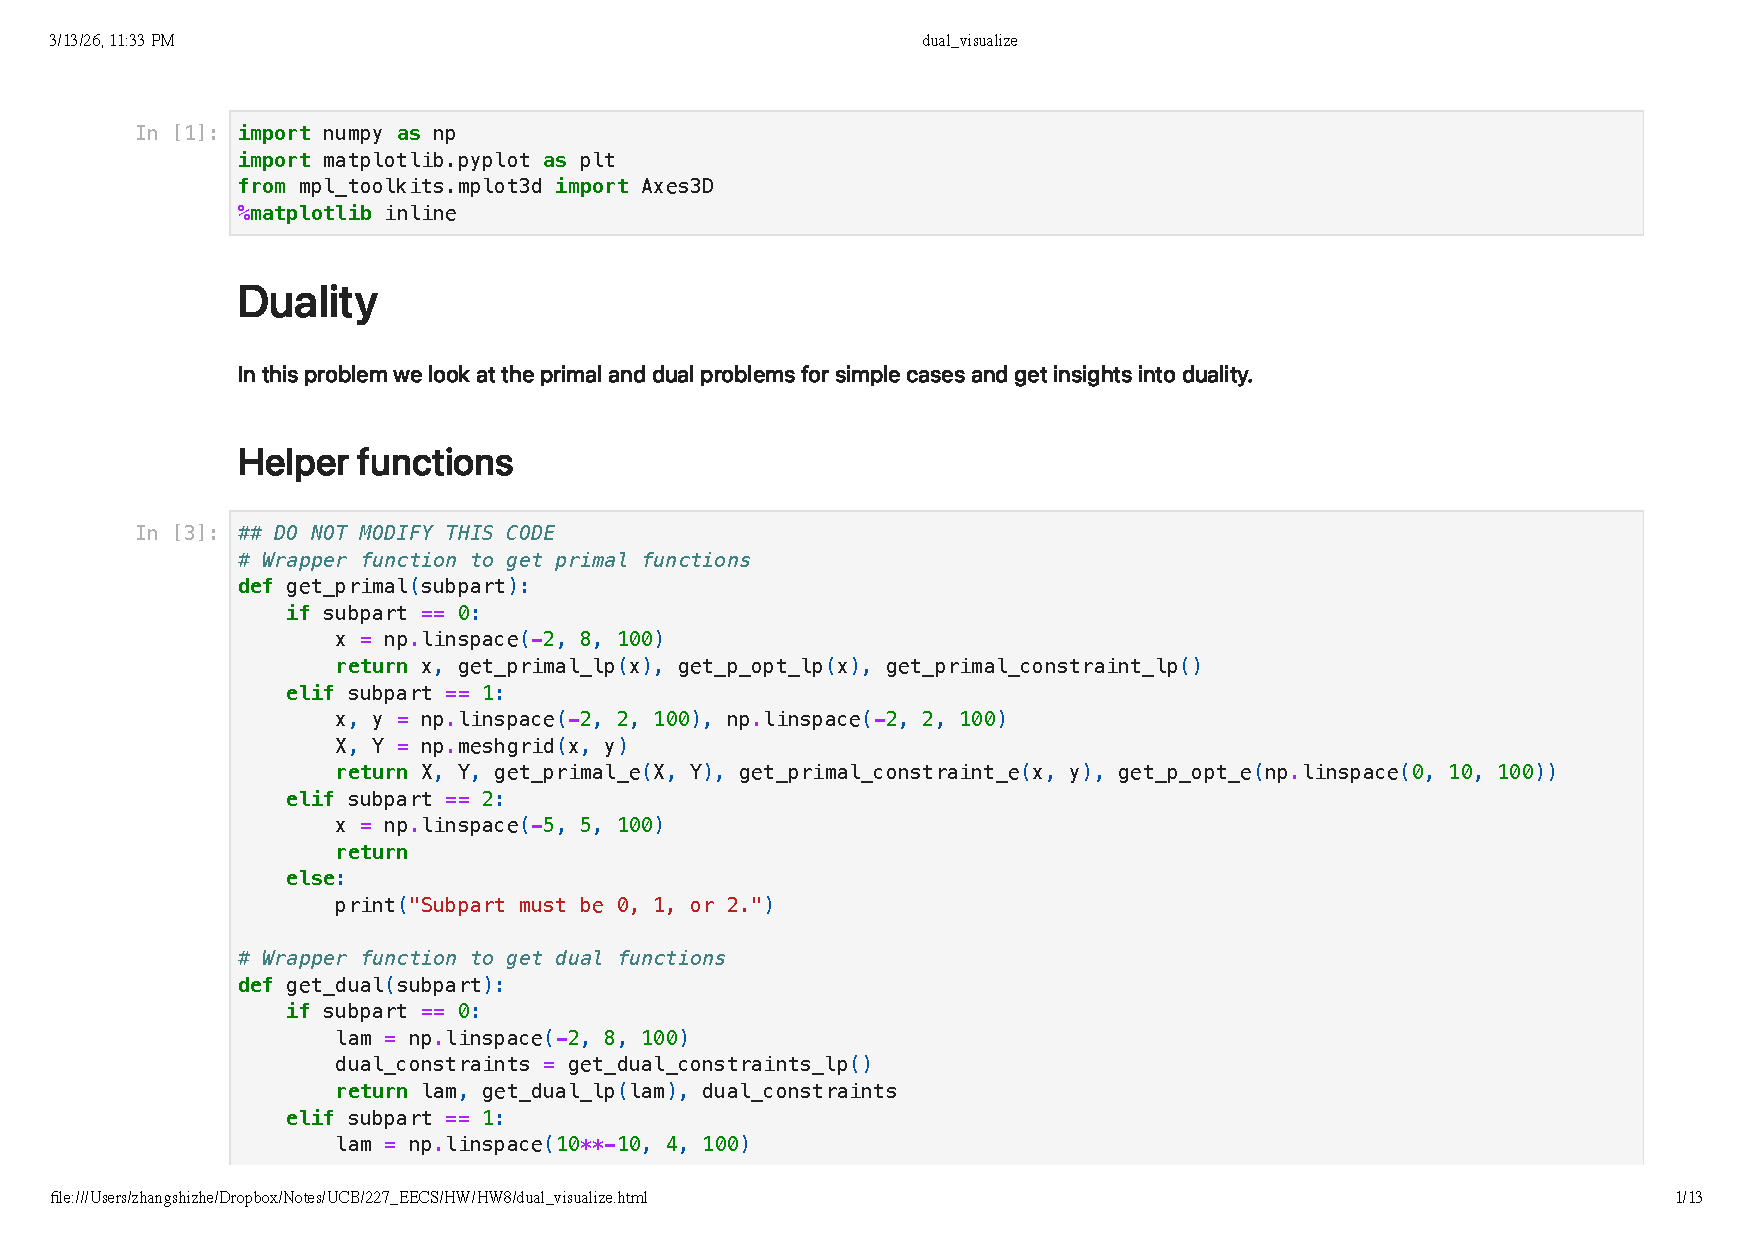
\includepdf[page=-]{dual_visualize.pdf}
%%%%%%%%%%%%%%%%%%%%%%%%%%%%%%%%%%%%%%%%%%%%%%%%%%%%%%%%%%%%
\newpage
\section*{5. Dual of an LP}

Consider the general form of a linear program:

\[
\min_{\vec{x}} c^\top \vec{x}
\tag{16}
\]

subject to

\[
A\vec{x}= \vec{b}.
\tag{17}
\]

\textbf{(a)} Write the Lagrangian function $L(\vec{x},\vec{\mu})$.

\textbf{(b)} Write the Lagrangian dual function $g(\vec{\mu})$.

\textbf{(c)} Write the dual problem.

\subsection*{Answer}

\textbf{(a)}

\[
L(\vec{x},\vec{\mu})
=
c^\top \vec{x}
+
\vec{\mu}^\top (A\vec{x}-\vec{b}).
\]

We can rearrange it as

\[
L(\vec{x},\vec{\mu})
=
(c^\top + \vec{\mu}^\top A)\vec{x}
-
\vec{\mu}^\top \vec{b}.
\]


\textbf{(b)}

\[
g(\vec{\mu}) = \inf_{\vec{x}} L(\vec{x},\vec{\mu}).
\]

\[
g(\vec{\mu})
=
\inf_{\vec{x}}
\left[
(c^\top + \vec{\mu}^\top A)\vec{x}
-
\vec{\mu}^\top \vec{b}
\right].
\]

If
$ c^\top + \vec{\mu}^\top A \neq 0, $
then the expression can be made arbitrarily negative by choosing 
$\vec{x}$ appropriately, so
$ g(\vec{\mu}) = -\infty.$

To obtain a finite value, we must have

\[
c^\top + \vec{\mu}^\top A = A^\top \vec{\mu} + c = 0.
\]

\[
g(\vec{\mu}) =
\begin{cases}
-\vec{\mu}^\top \vec{b}, & A^\top \vec{\mu} + c = 0 \\
-\infty, & \text{otherwise}.
\end{cases}
\]

\textbf{(c)}

\[
\max_{\vec{\mu}} -\vec{\mu}^\top \vec{b}
\quad
\text{s.t.}
\quad
A^\top \vec{\mu} = -c.
\]

%%%%%%%%%%%%%%%%%%%%%%%%%%%%%%%%%%%%%%%%%%%%%%%%%%%%%%%%%%%%
\newpage
\section*{6. Homework Process}

With whom did you work on this homework? List the names and SIDs of your group members.

NOTE: If you didn’t work with anyone, you can put “none” as your answer.

\subsection*{Answer}
none

\end{document}